\subsection{History of Computing}
Multiple devices have been used to aid computation for thousands of years like \eg  abacus, astronomical calenders,  differential analyser, etc. Charles Babbage, an English mechanical engineer, (considered the "father of the computer") originated the concept of a programmable computer in the early 19th century.

\par A computer is a machine that can be programmed to carry out sequences of arithmetic or logical operations automatically. Modern computers can perform generic sets of operations known as programs. The principle of the modern computer was proposed by Alan Turing in 1936. The fundamental concept of Turing's design was the stored program, where all the instructions for computing were stored in a memory. The next great advance in computing power came with the advent of the transistors, semiconductors, and integrated circuits. 

\par Machine code was the language of early programs, written in the instruction set of the particular machine, often in binary notation. Assembly languages were soon developed that let the programmer specify instruction in a text format, with abbreviations for each operation code and meaningful names for specifying addresses. 

\par With further development in software as well as hardware, Compiler languages were formulated. High-level languages made the process of developing a program simpler and more understandable, and less bound to the underlying hardware. These compiled languages allowed the programmer to write programs in terms that are syntactically richer, and more capable of abstracting the code, making it easy to target for varying machine instruction sets via compilation declarations and heuristics. Compilers harnessed the power of computers to make programming easier  by allowing programmers to specify calculations by entering a formula using infix notation.

\subsubsection{Introduction to C language}
C is a procedural programming language. It was initially developed at the AT \& T's Bell Laboratories of USA by Dennis Ritchie in the year 1972. It was mainly developed as a system programming language to write an operating system. The main features of the C language include: 
\begin{itemize}
    \item Portability (Machine Specific)
    \item Requires less lines of code than assembly language
    \item Procedural programming
    \item Middle level language   
    \begin{itemize}
        \item Direct access to memory through Pointers
        \item Bit manipulation using bitwise Operators
        \item Writing assembly code within C code
    \end{itemize}
    \item Popular choice for system level apps
    \item Wide variety of built in functions, standard libraries and header files.
\end{itemize}


\subsection{Elements of C Language}
Communicating with a computer involves speaking the language the computer understands. However, there is a close analogy between learning English and C language. Learning English comprises of learning the alphabets, then learn to combine those to form words, which in turn are combined to form sentences and then sentences are combined to form paragraphs.

\par Similarly, instead of straight-away learning how to write programs, we must first know what alphabets, numbers and special symbols are used in C, then how using them constants, variables and keywords are constructed, and finally how are these combined to form an instruction. A group of instructions would be combined later on to form a program. 

\subsubsection{The C Character Set}
A character denotes any alphabet, digit or special symbol used to represent information. \figref{CCharSet} shows the valid alphabets, numbers and special symbols allowed in C.

\begin{figure}[H]
    \begin{center}
        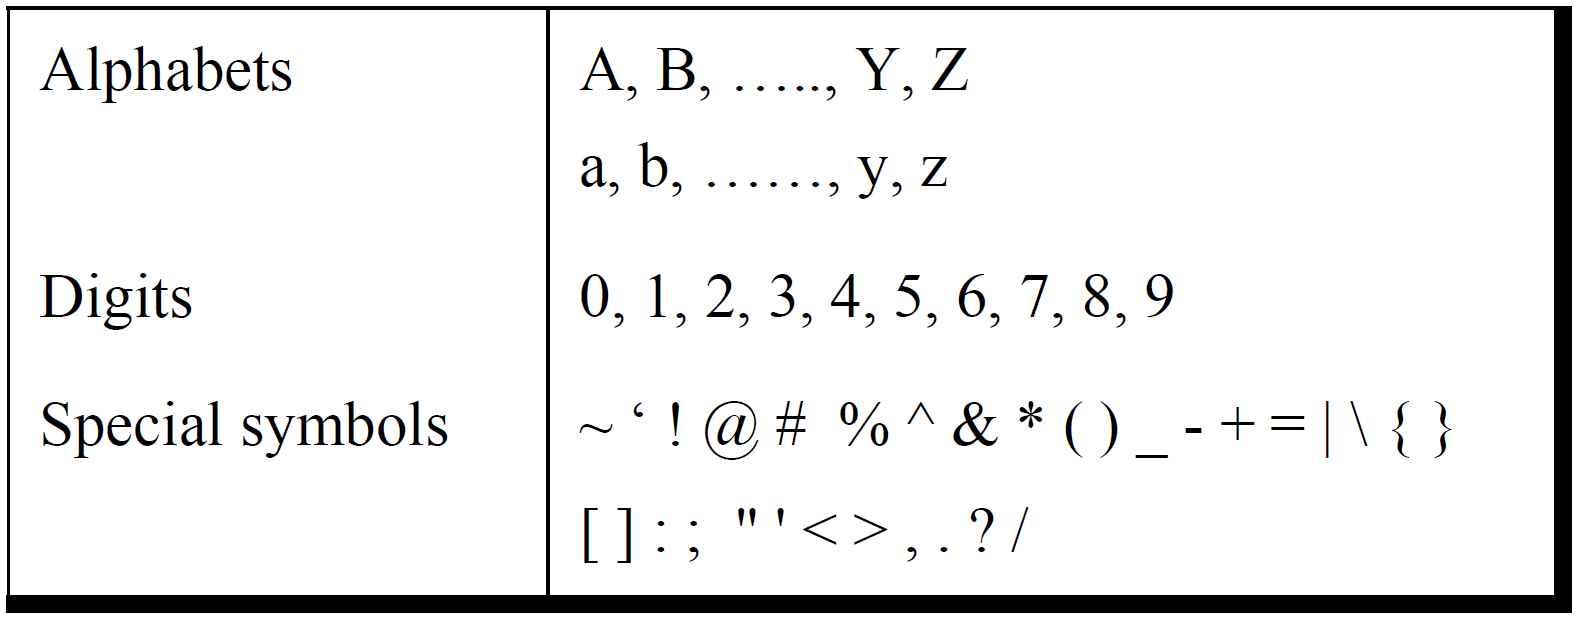
\includegraphics[width=\textwidth]{images/CCharSet.png}
        \caption{C Character Set}
        \label{CCharSet}
    \end{center}
\end{figure}

\subsubsection{Constants, Variables and Keywords}
The alphabets, numbers and special symbols when properly combined form constants, variables and keywords. Following sections explain 'constants' and 'variables' in detail. 

\subsubsection{C Instructions}
Constants, Variables and Keywords are combined to form an instruction to perform a certain functionality. There are basically three types of instructions in C:

\begin{enumerate}
    \item Type Declaration Instruction
    \item Arithmetic Instruction
    \item Control Instruction
\end{enumerate}

The purpose of each of these instructions is given below:
\begin{description}
    \item[Type declaration instruction] To declare the type of variables used in a C program.
    \item[Arithmetic instruction] To perform arithmetic operations between constants and variables.
    \item[Control instruction] To control the sequence of execution of various statements in a C program.
\end{description}
These instructions are decoded in the following sections.


\iffalse
\begin{itemize}
    \item Variables
    \item Operators
    \item Conditionals and Loops
    \item Functions
    \item Recursion
    \item Pointers and arrays
    \item Structure and union
\end{itemize}
\fi